	\subsection{Mountain Bike Suspension Concepts}
		The purpose of suspension on a mountain bike is to divert energy from bumps and rough features in a trail away from the rider to improve comfort and  performance by maintaining contact between the tires and the ground. This requires the use of a spring and damper, collectively known as a shock absorber, which allows the wheel to move away from the feature when it makes contact and make a controlled return once it has been passed.
	\subsubsection{Travel and Stroke} 
		\Gls{travel} is the distance which the bike's fork or frame allow the wheel to move in and upward direction. \Gls{stroke} is the distance that the shock absorber can compress before it bottoms out. \Gls{travel} is measured in inches or millimeters and can range from 80mm to 210mm. The amount of \gls{travel} which a bike has normally denotes which discipline it was intended for. Typically less suspension is required for endurance oriented riding and more for aggressive and rough situations.
		\begin{table}[h!]
		\centering
		\caption{Table of common suspension \glspl{travel} and intended disciplines}
		\label{tab:table1}
		\begin{tabular}{|c|cccc|}
			\hline
			Travel (mm)&Cross Country&Trail&Enduro&Downhill\\
			\hline
			80&\cellcolor[gray]{0.5}&&&
			\\
			100&\cellcolor[gray]{0.5}&&&
			\\
			120&\cellcolor[gray]{0.5}&\cellcolor[gray]{0.5}&&
			\\
			140&&\cellcolor[gray]{0.5}&\cellcolor[gray]{0.5}&
			\\
			160&&&\cellcolor[gray]{0.5}&
			\\
			180&&&\cellcolor[gray]{0.5}&\cellcolor[gray]{0.5}
			\\
			+200&&&&\cellcolor[gray]{0.5}\\
			\hline
		\end{tabular}
	\end{table}
	\begin{figure}[h!]
		\centering
		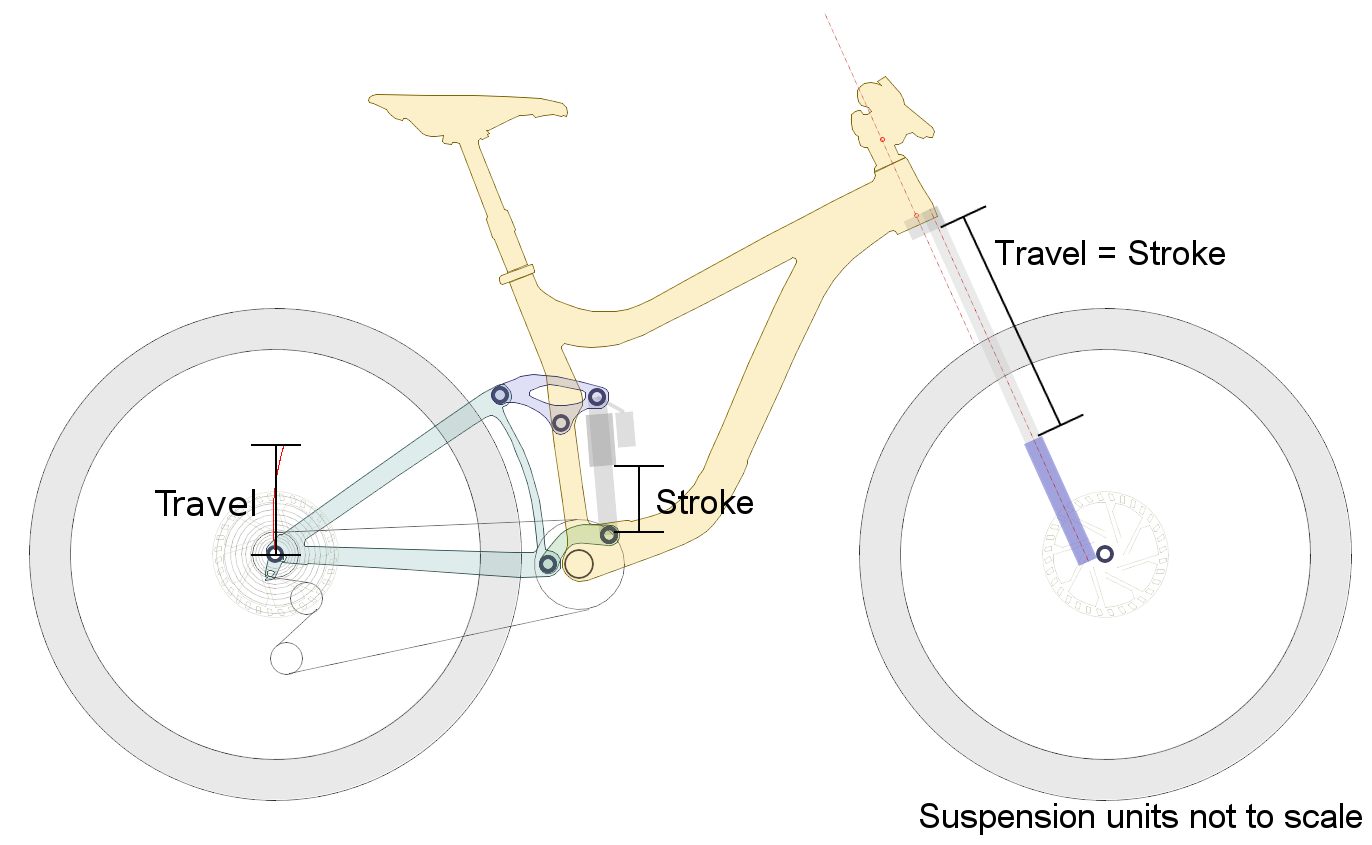
\includegraphics[width=12cm]{../images/reignschpath.PNG}
		\caption{Diagram showing travel and stroke on a full suspension bike}
		\label{fig:travelvsstroke}
	\end{figure}
	\subsubsection{Front Suspension}
		Front suspension commonly employs a linear telescoping shock absorber, known as a \gls{fork} due to it's dual sided construction. On nearly all suspension \glspl{fork} the \gls{stroke} is 1:1 with the potential travel of the wheel. Front suspension is found on all \gls{fs} and \gls{ht} bikes.
	\subsubsection{Rear Suspension}
		Rear suspension uses a shock absorber much smaller than a \gls{fork} and does not operate on a 1:1 ratio. Bike frames incorporate one or more pivot points and linkages which allows the wheel to move and act as multipliers for the suspension. Rear ratios are expressed as n:1 where n is the distance the rear wheel moves for every 1mm the shock compresses through its stroke. Though this is only the average leverage ratio for the entire travel.
		\\\\
		As all rear suspension designs are different and the rear wheel must rotate around the main pivot, or in some cases virtual pivot, as opposed to moving linearly, the frame will behave differently through its travel and depending on the type of \gls{shock} it is using. Because of this the average ratio is normally dismissed in favour of a leverage curve.
		\begin{figure}[h!]
			\centering
			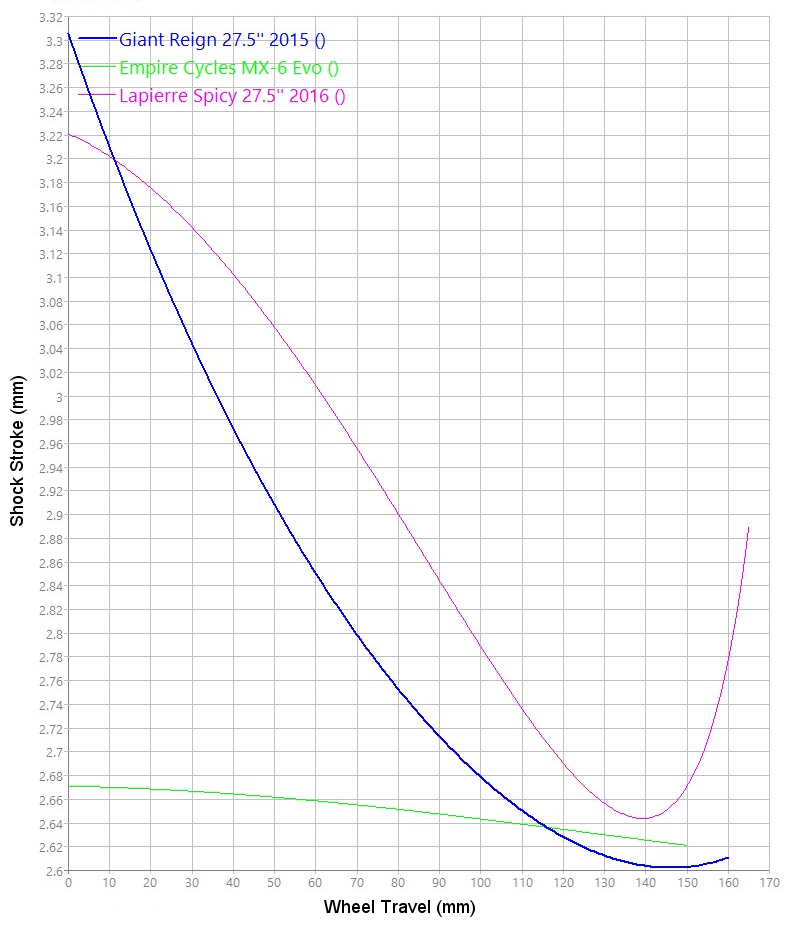
\includegraphics[width=10cm]{../images/3_bike_lev_ratio.jpg}
			\caption{Leverage curves of three modern suspension designs}
			\label{fig:3_bike_lev_ratio}
		\end{figure}
		\\\\
		Figure \ref{fig:3_bike_lev_ratio} shows the leverage curves of three modern suspension designs. Each of these designs has between 150mm and 170mm of travel and uses the 27.5 inch wheel size however it can be seen that their suspension hosts drastically different characteristics. 
		\\\\
		The \gls{vpp} design of the Giant Reign (shown blue) has an initial falling rate, meaning the \gls{shock} can be compressed easily, but slows down and even rises slightly towards the end of its travel. This means the suspension will feel soft most of the time but feel stiffer on large compressions. This is emphasised by the \gls{horst} system of the Lapierre Spicy (shown magenta) which has a large rise at the end of its travel.
		\\\\
		In contrast, the curve of the \gls{singlepiv} Empire MX-6 Evo (shown green) is considered linear. This is due to the MX-6 having only one pivot and swinging arm, as opposed to multiple pivots and linkages of the \gls{vpp} and \gls{horst} designs, so there is an almost direct input from the rear wheel to the \gls{shock}.
		\\\\
		For this project the bike used for development and testing of the application will be a 2015 Giant Reign, shown on figure \ref{fig:3_bike_lev_ratio} in blue, as there will be constant access to it during the project. The frame uses Giant's Maestro\texttrademark suspension system which is a variation of \gls{vpp}. Like all \gls{vpp} systems Maestro uses two links, an upper and lower, to create a virtual main pivot point, however unlike other \gls{vpp} systems, Maestro creates its virtual pivot as close to the rear of the frame as possible. Indicated by the red circle in figure \ref{fig:maestro}, the location of this virtual pivot is unique and, many believe, creates the most efficient suspension system on the market.
		\begin{figure}[h!]
			\centering
			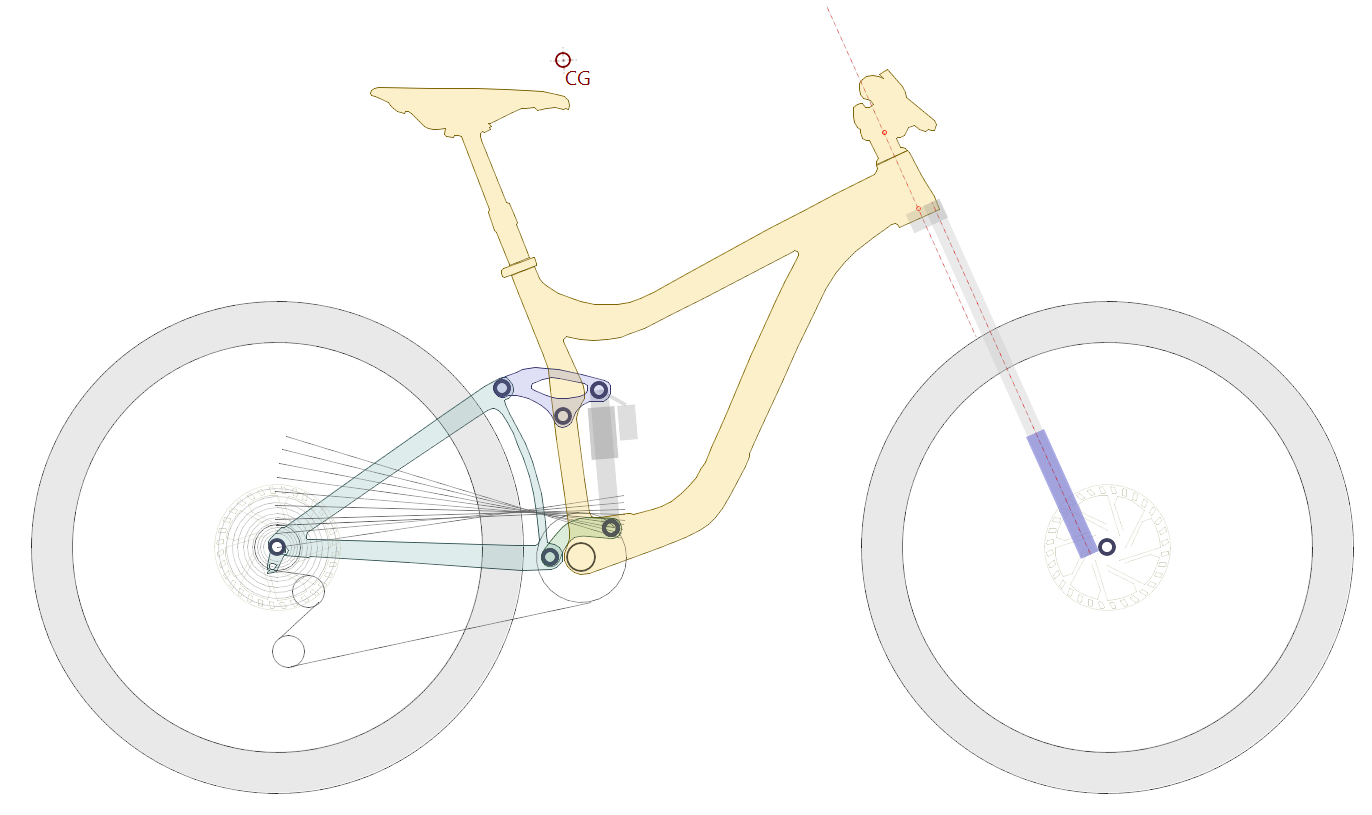
\includegraphics[width=12cm]{../images/reignsch.PNG}
			\caption{Maestro suspension}
			\label{fig:maestro}
		\end{figure}
	\subsubsection{Sag}
		\Gls{sag} is the amount that the suspension sits into its travel when the rider is in their neutral position, it is calculated using the rider's weight, available \gls{travel}, and intended riding style. \Gls{sag} is required so the suspension is able to drop into holes as well as soak up bumps. 
		\\\\
		To adjust \gls{sag}, the stiffness of the spring must be adjusted as required. This is done by changing the air pressure when using an air spring or replacing the coil and adjusting the spring pre-load on traditional coil \glspl{shock}. Depending on discipline and the amount of \gls{travel} the bike has, \gls{sag} can vary between 15\% and 40\% of the available travel though is commonly set between 25\% and 35\% for the average rider. 15\% and 40\% are reserved for competitive situations. 
	\subsubsection{Damping}
		Suspension damping is carried out by forcing oil within the shock absorber through an arrangement of holes in the absorber's damping circuit. Reducing the size or number of holes making the travel of oil through the circuit slower and therefore increases the damping effect making compression or rebound slower.
	\paragraph{Compression Damping} 
		This is applied while the shock absorber is being compressed. More damping forces the wheel to remain in contact with the ground which makes the suspension feel stiffer. Too much compression damping can make the suspension too stiff so it does not soften bumps or rough sections correctly. Too little can cause the suspension to "blow through" its travel prematurely potentially leaving none when it would be required.
	\paragraph{Rebound Damping}
		This is used to control the speed at which the shock absorber extends once it has been compressed. An optimal setting will allow the suspension to track the ground, returning after a bump as well as dropping into any holes. Too much \gls{rebounddamping} causes the suspension to return slowly and sometimes pack down meaning the absorber gradually runs out of travel. Too little can cause the suspension to buck the rider and lead to an accident.
	\paragraph{High and Low Speed Damping} 
		Depending on the manufacturer and model of the shock absorber, the unit can include up to two adjustable speeds for each damping circuit making four adjustable damping settings in total. High speed adjustments are used in high impact situations such as large jumps or drops, compression tends to be set softer to remove impact and rebound slower so rider has time to recover and the bike is not made unstable.
		\\\\
		Low speed adjustments are used against small movements such as rider weigh shifts or long, slow compressions. Optimally compression is set stiffer as this type of feature can use a lot of travel and \gls{rebounddamping} set faster to deal with multiple features in quick succession.
	\subsubsection{Optimal Setup}
		Although setups will vary between rider, suspension system, and discipline there are some key aspects which all riders should aim to achieve. Sag should be set to an appropriate measurement by adjusting the air pressure on air \glspl{shock} or spring rating on coil \glspl{shock}. Compression damping should feel soft and soak up bumps efficiently without excessive bottoming out. Rebound damping should be set to return as fast as possible without bucking the rider, this is normally in the middle of the two extremes of setting with a slight bias to the fast option.